%!TEX root = Projektdokumentation_ClockPendulumAnalyzer.tex
\newcommand*{\risk}[2]{
    \begingroup
    \ifnum #1>#2
    \cellcolor{red}
    \fi
    \endgroup
}

\section{Risikomanagement}
    In diesem Kapitel werden allfällige Risiken identifiziert, bewertet und verwaltet. 
    \subsection{Risikobewertung}
    Im Projekt wurden folgende Risiken (Tabelle \ref{tab:risks}) identifiziert und anhand der Auswirkung und Eintrittswahrscheinlichkeit bewertet. Die Bewertungsmatrix in Bild \ref{fig:riskmatrix} zeigt die möglichen Risikowerte auf.
    \begin{table}[H]
        \centering
        \begin{tabular}{|l|l|c|c|c|}
            \hline
            \textbf{Nr} & \textbf{Risiko} & \textbf{Auswirkung} & \textbf{Eintrittsw'keit} & \textbf{Risikowert}\\ \hline
            1 & Fehlerhafte Implementation & 2 & 2 & \cellcolor{yellow}4\\ \hline
            2 & Teammitglied fällt aus & 2 & 2 & \cellcolor{yellow}4\\ \hline
            3 & Auftraggeber fällt aus & 1 & 1 & \cellcolor{green}1\\ \hline
            4 & Teamdifferenzen & 2 & 1 & \cellcolor{green}2\\ \hline
            5 & Verlust des Programmcodes & 3 & 1 & \cellcolor{yellow}3\\ \hline
            6 & Motivation verschwindet & 2 & 1 & \cellcolor{green}2\\ \hline
            7 & Fehlende Kommunikation mit Stakeholder & 3 & 1 & \cellcolor{yellow}3\\ \hline
            8 & RTC Module kommen zu spät & 3 & 1 & \cellcolor{yellow}3\\ \hline
            9 & Eingeschränkte Debugging Funktionalität & 2 & 3 & \cellcolor{red}6\\ \hline
            10 & Hardwareteile gehen kaputt & 2 & 2 & \cellcolor{yellow}4\\ \hline
            11 & Projektreport geht verloren & 3 & 1 & \cellcolor{yellow}3\\ \hline
            12 & Testuhr geht verloren & 2 & 1 & \cellcolor{green}2\\ \hline
            13 & Umsetzung entspricht nicht den Erwartungen & 3 & 2 & \cellcolor{red}6\\ \hline
        \end{tabular}
        \caption{Tabelle der identifizierten Risiken}
        \label{tab:risks}
    \end{table}
    
    \begin{figure}[H]
        \centering
        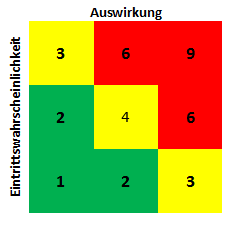
\includegraphics{Risikomatrix.png}
        \caption{Risikobewertung in einer 3x3 Matrix}
        \label{fig:riskmatrix}
    \end{figure}
    
    \clearpage
    \subsection{Massnahmenkatalog}
    Die Risiken mit einem Wert von 6 oder 9 werden als kritisch empfunden und erhalten eine Auflistung von Massnahmen gegen Auswirkung und Eintritt (Tabelle \ref{tab:arrangements}).
    \begin{table}[h]
        \centering
        \begin{tabular}{cp{7cm}p{7cm}}
            \textbf{RisikoNr} & \textbf{Massnahmen gegen Auswirkung} & \textbf{Massnahmen gegen Eintrittsw'keit}\\ \hline
            9 & \tabitem Alternative IDE für Debugging Zwecke & \tabitem Persönliche Präferenzen zurückstellen \\ \hline 
            13 & & \tabitem regelmässiges Reporting an die Stakeholder\\
            & &\tabitem gutes Requirementsengineering\\ \hline
            
        \end{tabular}
        \caption{Massnahmen gegen kritische Risiken}
        \label{tab:arrangements}
    \end{table}